\documentclass[11pt]{article}

% Packages

\usepackage{amsmath}
\usepackage{amssymb}
\usepackage{color}
\usepackage{graphicx}

% Style

\newcommand{\Keywords}[1]{\vspace{12pt}\par\noindent
{\small{\bf Keywords\/}: #1}}
\renewcommand{\thesection}{\Roman{section}} 
\renewcommand{\thesubsection}{\thesection.\Alph{subsection}}
\renewcommand{\thesubsubsection}{\thesubsection.\arabic{subsubsection}}
\renewcommand{\thetable}{\Roman{table}}

% Helpers

\newcommand{\E}[1]{\times10^{#1}}
\newcommand{\braket}[2]{\left<#1\middle|#2\right>}
\newcommand{\iso}[2]{$^{#2}\mathrm{#1}$}
\newcommand{\tild}[0]{\sim\!\!}
\newcommand{\REF}[0]{\colorbox{yellow}{REF}}
\newcommand{\water}[0]{$\mathrm{H_2O}$}

\begin{document}

\title{The Reactivity Effects of Flibe Impurities in FHRs}
\author{Jeffrey E. Seifried \and Raluca O. Scarlat \and Per F. Peterson\footnote{Email: peterson@nuc.berkeley.edu} \and Ehud Greenspan \\
\em University of California Berkeley\\
\em Department of Nuclear Engineering\\
\em 4155 Etcheverry Hall, MC 1730\\
\em Berkeley, CA 94720, USA
}
\date{}
\maketitle

\begin{abstract}
    This work quantifies the reactivity impact of 53 impurities within the primary coolant for thermal spectrum Fluoride-Salt Cooled High-Temperature Reactors (FHR).
    It does so, not by assuming a mixture of impurities, but by individually assessing the impact of each impurity per amount present -- so called ``specific reactivity worths''.
    Two approaches are taken to making these estimates, one using the new KSEN tool in MCNP6.1 and a more traditional one using spectrum-collapsed absorption cross-sections.
    The KSEN tool is shown to be very effective at this procedure.
    The utility of these specific reactivity worths is demonstrated by estimating the impact of flibe impurities upon the coolant temperature coefficient of reactivity, the system excess reactivity, and the achievable discharge burnup for an example FHR.
    Some discussion is also provided on the available detection and removal techniques for important impurities.

    \Keywords{flibe, sensitivity, adjoint, thermal spectrum reactor, reactivity worth, neutron poisons, molten salt}
\end{abstract}

\pagebreak

\section{Introduction}
\label{sec:intro}

Liquid fluoride salt cooled reactors were first proposed in 2000 by Peterson, Forsberg, and Pickard, under the title of Advanced High Temperature Reactors (AHTR) \cite{forsberg2003msc}, and they were later renamed to Fluoride-Salt Cooled High-Temperature Reactors (FHR) \cite{scarlat2013csf}.
FHRs combine the coated particle (TRISO) fuel and graphite reflectors of gas-cooled reactors \REF with the coolant of molten salt reactors (MSR) \REF, thus taking advantage of a robust solid fuel and a liquid salt coolant which has excellent thermophysical properties as reactor coolant.
The two technologies have been extensively studied and when combined they provide a large number of safety and economic advantages over other types of nuclear reactors \REF.

Several variants of FHR designs are being developed in the US and China.
UC Berkeley is developing the pebble bed FHR (PB-FHR), with randomly packed pebble fuel that allows for online refueling.
The pebbles have a graphite core and a thin annular fuel zone, and are $3cm$ in diameter  \REF.
Oak Ridge National laboratory has two designs that use plate fuel, the AHTR, and the SmAHTR  \REF.
The Chinese Academy of Sciences is building a $2MW$ test reactor, with pebble fuel arranged in a fixed lattice.
The pebble fuel diameter is $6cm$, same as for the high temperature gas-reactor \REF.

Among the large number of liquid fluoride salt mixtures that have been studied as part of the MSR program, $LiF-2 BeF_2$ (flibe) was selected as the coolant of choice due to its thermophysical, chemical, and neutronic properties.
Its high volumetric heat capacity allows for low volumetric flow rates and consequently compact equipment can be used.
Its relatively low viscosity further contributes to a pumping power that is negligible with respect to the reactor thermal power.
It has a moderately high melting point of $450^\circ C$ and a very low vapor pressure up to temperatures of $1200^\circ C$ and above, which enable operation of a single phase reactor at atmospheric pressure with very high margin to boiling.
Among other fluoride salt mixtures flibe has the highest moderating ratio, allowing a broad range of reactor cores to have negative primary coolant temperature coefficients of reactivity.
The same neutronic properties also allow for the best fuel utilization performance among other fluoride salts \cite{williams2006acm}.
For these same reasons, flibe remains the coolant of choice for FHRs.

Flibe was originally selected as a reactor coolant and fuel solvent for molten salt reactors, in which the fuel and all of its fission products are dissolved in the coolant.
Flibe is therefore by design a great solvent for a large class of elements.
Thus the primary coolant on the one hand provides an additional barrier to radionuclide release in the event of fuel failure, and on the other hand has high affinity for impurities.
FHRs are designed to operate with a clean salt, so the effect of impurities must be well understood.
The presence of impurities can have an effect on corrosion of metallic and ceramic components, on salt chemistry control, on circulating activity due to neutron activation of impurities, on reactivity characteristics, and in extreme cases of contamination on the thermophysical properties of the fluid.

This study investigates the reactivity effects of impurities in the flibe primary coolant of FHR.
The importance of impurities on the neutronics of new reactor technologies was an important lesson learned from the High Temperature Engineering Test Reactor (HTTR) of the Japan Atomic Energy Agency.
The presence of trace boron within the graphite blocks of the HTTR, which was neglected in simulations, is thought to account for the bias of $+1.5\%$ to $+2.1\%$ in the predicted multiplication factor during the initial critical configuration.
Consequently, the number of fuel columns necessary for criticality that was under-predicted by $16\%$ \cite{bess2010esu}.

During the MSRE project at ORNL, work was done to measure the impurities present in the clean flibe salt and propose quantitative limits for salt purity.
These limits also took into consideration the operational requirements of the experiment, the likelihood of contamination from each impurity, and the availability and cost of salt cleaning techniques.
The limits were based upon the role that impurities played in reactivity effects, activation, corrosion, and chemistry \cite{shaffer1971phs}.
With this holistic approach, the limits were somewhat optimized to efficiently target the worst-acting impurities while allowing any innocuous impurities to remain.

A similar approach should be adopted for the purity of flibe in FHR, and this study provides the analysis of the reactivity effects in support of this objective.
We quantify here the reactivity impact as a function of concentration of each of the salt impurities, which includes penalties upon the coolant temperature coefficient of reactivity, excess reactivity, and achievable burnup.
These penalties, combined with chemistry effects of impurities, purification limits, and other design constraints can be used to generate limits for salt purity for FHRs.
The generation of activity in the primary coolant due to activation of impurities external to the fuel particles is not analyzed in this study, but merits future work.
Section \ref{sec:impurities} lists the flibe impurities which are considered.
Section \ref{sec:methodology} describes the approaches used for quantifying the reactivity effect of those impurities.
Section \ref{sec:results} tabulates those reactivity effects.
Section \ref{sec:discussion} discusses the limitations of the methodology used, demonstrates the utility of the reactivity effects, and discusses existing strategies for detection and removal of impurities.

\section{Impurities considered}
\label{sec:impurities}

There are a number of ways in which impurities can be introduced to the salt.
Before it enters a reactor, the salt is manufactured and comes into contact with containers during processing, transport, and storage.
Once loaded into the reactor, additional contamination can occur; elements may leach out of the metal alloy or ceramic structural materials that come into contact with the salt.
For example, chromium metal alloys will introduce chromium into the salt and graphite often has helium, boron, and uranium impurities which may transport into the salt.
Other elements, such hydrogen, zirconium, cerium, and europium may be intentionally added to control the fluorine potential of the salt and limit its corrosion of the structural materials.

The ORNL MSRE work \cite{shaffer1971phs} documented the presence of 31 impurities in clean flibe -- water, 15 rare earth elements, and 15 other elements.
Recent flibe impurity measurements by MIT, using neutron activation analysis on flibe manufactured at University of Wisconsin detected a total of 43 impurities, 22 of them being additional impurities that hadn't been previously documented by the MSRE work \cite{ames2013tea}.
Based on these two studies, we consider here a total of 53 potential flibe impurities: \water{}, B, Na, Mg, Al, Si, S, Cl, K, Ca, Sc, Ti, V, Cr, Mn, Fe, Co, Ni, Cu, Zn, As, Se, Br, Rb, Sr, Y, Zr, Mo, Cd, Sb, Cs, Ba, La, Ce, Pr, Nd, Sm, Eu, Gd, Tb, Dy, Ho, Er, Tm, Yb, Lu, Hf, Ta, W, Au, Hg, Th, and U.
Strategies are still under development for chemistry control and the final structural materials have not been selected, so additional elements may require study in the future.
All elements that are introduced by the chemistry control system need to be considered, as well as all elements present in the structural materials that come into contact with the salt, because, depending on the fluorine potential of the salt, they may transport into the salt.
Currently, the two metal alloy candidates for the reactor vessel, piping, and other internal components are Hastelloy N (C, Cr, Mn, Mo, Ni, Si, Fe) and stainless steel 316 (C, Cr, Cu, Mn, Mo, N, Ni, P, S, Si, Fe) \REF.

This paper only considers impurities which might initially reside in the salt, or might migrate from other components into the salt.
Although parasitic capture anywhere in the system can reduce excess reactivity and achievable burnup, only impurities within the salt can affect coolant void coefficients of reactivity.
Impurities elsewhere may also alter the Doppler coefficient of reactivity of those regions and the achievable burnup, but this is highly system specific and is considered outside the scope of the current work.
Impurities which are present at such a high concentration that flux spectra are perturbed significantly are also not considered; such concentrations are not likely to be reached due to salt purity limits set by chemistry or neutronics considerations.
Transmutation of impurities is not considered -- all elements are presumed to be present at their natural abundances.
While irradiation decreases the capture probability for most elements, it is possible for their activation (or fission) products to possess higher absorption cross-sections.
The effects from these transmutation daughters will vary with operation and are expected to bring only moderate deviations.
Therefore, this analysis can be considered applicable primarily to coolant which has experienced a small fluence, for example, fresh coolant in a commercial reactor, or fresh coolant over the entire lifetime of a test reactor.

\section{Methodology}
\label{sec:methodology}

The reactivity effects of these impurities are quantified by performing a sensitivity analysis upon a characteristic PB-FHR pebble unit cell, whose dimensions and compositions are extracted from recent design work on the PB-FHR fuel \REF.
The unit cell is filled with a BCC lattice of $3cm$ OD pebbles with mirror reflection and $40\%$ salt by volume.
The $500\mu m$ diameter TRISO fuel kernels are composed of $UO_{1.5} C_{0.5}$ enriched to $19.9w/o$ \iso{U}{235} and spaced to bring about a carbon-to-heavy-metal atomic ratio of $300$.
Cross-sections and thermal scattering kernels for all materials are broadened to $900K$ and the salt is given a mass density of $1962.8 kg/m^3$.
\iso{Li}{6} is depleted to $50wppm$ (on a lithium mass basis) within the salt.

The KSEN sensitivity tool in MCNP6.1 estimates the fractional change in a system's multiplication factor due to a fractional change of a cross-section or material density \cite{lanl2013mcnp6,kiedrowski2013abk}.
From this, the specific reactivity worth -- the reactivity penalty incurred per weight fraction increment of an impurity -- can be calculated as:
\begin{equation}
    \frac{\partial\rho}{\partial w}
    = \frac{1}{k} \frac{\sum_x{S_{i,x}}}{w_i}
    ,
\end{equation}
where $i$ denotes a constituent, $x$ denotes a nuclear reaction type, and $\rho$, $w$, $k$, and $S$ are the reactivity, weight fraction, multiplication factor, and multiplication factor sensitivity coefficient.
The power of sensitivity methods is that they can isolate the individual impact of many impurities with a single transport calculation.
However, KSEN requires each impurity to be present in a model.

Each impurity must be added to the salt at a concentration which allows for measurable interaction with neutrons -- in order to limit Monte Carlo counting uncertainties -- but which doesn't excessively perturb the system -- so that self-shielding among impurities is minimized and so that flux and importance spectra do not differ from that of reactor operation with clean salt.
Some verification for this last requirement is provided in Section \ref{sec:discussion}.
Concentrations (on a salt mass basis) are chosen to match the Maxwellian-averaged neutron absorption macroscopic cross-section of $0.1wppm$ \iso{Li}{6} (on a lithium mass basis) \cite{mughabghab2003tnc} \cite{holden1999tdw}, where the FHR \iso{Li}{6} concentration at start-up is likely to be $50wppm$ \REF.
While these so called ``thermal poison equivalents'' ignore the effects of moderation and resonance capture, an accurate sensitivity analysis only requires that impurities are added to the model at concentrations of the correct order of magnitude.
Table \ref{tab:thermalLimits} tabulates thermal poison equivalents for 52 impurities.
A thermal poison equivalent for water would not be meaningful since it acts primarily as a moderator; instead  Table \ref{tab:thermalLimits} includes the ORNL MSRE concentration limit for water \cite{shaffer1971phs}.

Specific reactivity worths can also be approximated with a simpler, less accurate method which doesn't require the explicit addition of impurities to the model.
If scattering, fission, and leakage effects of impurities are ignored and the importance can be approximated to be spatially and spectrally uniform, only the spectrum-collapsed absorption cross-section is required.
A single transport calculation can extract these cross-sections from the pebble unit cell filled with clean salt and specific reactivity worths can be calculated as:
\begin{equation}
    \frac{\partial\rho}{\partial w}
    \approx \frac{\braket{\sigma_i^{abs}}{\psi}}{k} \frac{\rho_m N_{avo}}{M_i}
    ,
\end{equation}
where $\sigma^{abs}$, $\psi$, $\rho_m$, $N_{avo}$, and $M$ are the microscopic neutron absorption cross-section, neutron flux, material mass density, Avogadro's number, and constituent atomic mass.
The inner product notation $\left<\square\right>$ indicates integration over space, direction, and energy of the neutron phase-space.
Because the approach doesn't require estimation of the adjoint distribution, it is significantly more computationally efficient.
Results for both the sensitivity and absorption approaches are provided and compared in the Section \ref{sec:results}.

Tm and Yb are excluded from direct evaluation of specific reactivity worths due to their absence in the ENDF/B-VII.0 evaluated nuclear data library \cite{chadwick2006endf70}.
Consequently, specific reactivity worths for Tm and Yb are approximated as those of Sc and Cs, respectively, due to their similar neutron poison equivalents in Table \ref{tab:thermalLimits}.
\iso{Ta}{180} and \iso{W}{180} are also absent from ENDF/B-VII.0, but since they make up only $\tild 0.01a/o$ and $\tild 0.1a/o$ of their elements' natural abundances, respectively, no special corrections are performed.
It is worth noting that Tm, Yb, \iso{Ta}{180}, and \iso{W}{180} are all present in ENDF/B-VII.1 \cite{chadwick2011endb71}.
Because U resides in the fuel and spatial discrimination of sensitivities is not yet implemented in MCNP6.1, a sensitivity-based estimate could not be derived for U.

\section{Results}
\label{sec:results}

In Table \ref{tab:sensitivityWorths}, specific reactivity worths derived from sensitivity analysis are tabulated for 52 flibe impurities (all but U).
When uncertainties of results are greater than $20\%$, they are colored red; when they are between $10\%$ and $20\%$, they are colored blue; otherwise they are colored black.
Correlation coefficients of $0$, $+1$, and $-1$ are conservatively assumed for addition, multiplication, and division of random variables, respectively.
For a point of reference, the specific reactivity worth for \iso{Li}{6} was found to be $-224.2\pm0.1pcm/wppm$.

Table \ref{tab:sensitivityWorths} only shows the effect of elemental impurities which are assumed not to displace flibe components.
If one wishes to consider the fluoride associated with an impurity along with the flibe component(s) it displaces, Table \ref{tab:flibeWorths} may be used.
For this table, all flibe components are at the stoichiometric proportions of $50wppm$ \iso{Li}{6} flibe.

In Table \ref{tab:absorptionWorths}, specific reactivity worths derived from spectrum-collapsed absorption cross-sections are tabulated for all 53 flibe impurities (including U) and flibe itself.
Agreement with Table \ref{tab:sensitivityWorths} and Table \ref{tab:flibeWorths} is good, however estimates for \water{} and flibe -- compounds which serve as strong moderators -- are estimated to be negative when they are known to be positive because the system possesses a negative coolant void coefficient of reactivity.
The absorption approach estimates the \iso{Li}{6} specific reactivity worth to be $-170.32\pm0.04pcm/wppm$ -- $24\%$ lower in magnitude than that estimated with sensitivity analysis.
Overall, estimates are non-conservatively under-predicted in magnitude by $\tild 20\%$.

\section{Discussion}
\label{sec:discussion}

The total reactivity penalty from the 53 impurities can be calculated directly from the clean and contaminated state multiplication factors as $-0.229\pm0.005 \%\Delta\rho$.
By comparing this penalty to that derived from summation of the estimated penalty from each impurity, the accuracy of the two approaches for estimating specific reactivity worths can be assessed.
The sensitivity approach estimates a total penalty of $-0.225\pm0.03 \%\Delta\rho$ which is low by $1.8\pm16\%$ ($0.1$ standard deviations); the absorption approach estimates a total penalty of $-0.20684\pm0.00003 \%\Delta\rho$ which is low by $10\pm2\%$ ($5$ standard deviations).
In spite of the lesser accuracy of the absorption approach, it estimates specific reactivity worth at a far greater precision than the sensitivity approach.
If the approach is used in the future due to this large advantage in computational efficiency, it is recommended that a $1.25\times$ multiplier be applied to its estimates before they are used.
This multiplier is crude and does not match the total reactivity effect, but performs well for most impurities.

Using specific reactivity worth estimates from Table \ref{tab:sensitivityWorths} or Table \ref{tab:absorptionWorths}, the required precision of detection and removal techniques for each impurity can be approximated.
For example, if the reactivity worth of Cd is required to be less than $-20pcm$, its concentration must be known to a precision of roughly $0.1wppm$.
Table \ref{tab:precision} tabulates these values for all 53 impurities.

As an impurity, \water{} acts primarily as a moderator -- a quality it inherits from H.
The specific reactivity worth of H is estimated to be $+3.0\pm0.2 pcm/wppm$ (or $-0.35772\pm0.00009pcm/wppm$ when neglecting moderation) and that of O is vanishingly small, so neither the compound nor its constituents should be limited from reactivity concerns.
The same should be said for He and C, two light low-capture elements, and Ar, which has a capture cross-section similar to Ce: \water, He, C, Ar, and Ce should not be limited due to neutron absorption effects.

The explicit addition of 53 impurities for the sensitivity-based estimation of specific reactivity worths perturbs the system from the clean state.
It is important that this perturbation be small so that impurity reactivity effects do not saturate and therefore remain linear.
One way of measuring the degree of perturbation is to compare flux spectra within the salt before and after the impurities are added.
Figure \ref{fig:fluxSpectra}, shows that the spectrum suffers only small changes upon adding the impurities.
When water is subtracted from those impurities, only (mostly) poisoning impurities remain and the thermal flux is depressed only slightly by the increased capture.

Sensitivity coefficients are calculated by folding distributions of the adjoint and flux with material cross-sections.
Therefore, any system whose flux and adjoint spectra (and spatial and directional distributions) match those of this work, would have identical values for Table \ref{tab:sensitivityWorths}, Table \ref{tab:flibeWorths}, and Table \ref{tab:absorptionWorths}.
Although exact matching of spectra is difficult, FHRs, MSRs, and other systems with an abundance of flibe and graphite can have similar spectra.
Even when only approximate matching can be achieved, the relative rankings of specific reactivity worths are unlikely to change.

Specific reactivity worths can be used to guide the salt cleaning and chemistry control strategy.
Upon determining a maximum permissible reactivity limit, a number of impurity mixtures whose summed reactivity effect is below that limit can be defined.
Acceptable mixtures can be down-selected by considering the amount of each impurity which is expected and the difficulty of removing each impurity.
Further down-selection would occur after performing corrosion and activation studies.
As in any design problem, otherwise uncorrelated performance metrics will have to be balanced.
In this case, the balance is struck between reactivity-related performance, corrosion performance, activation performance, and investment in salt cleanup.
Reactivity-related performance can be determined from several perspectives, but three are discussed in this work: the coolant temperature coefficient of reactivity, the initial excess reactivity and critical configuration, and the achievable burnup.

\subsection{Effect on coolant temperature coefficient of reactivity}
\label{sec:exampleCoefficient}

The coolant temperature coefficient of reactivity ($\alpha_{c,T}$) can be split into two coefficients -- the coolant void coefficient of reactivity ($\alpha_{c,V}$) and the coolant Doppler coefficient of reactivity ($\alpha_{c,D}$) -- and most flibe impurities will affect only the former.
In under-moderated systems, neutron moderation within the coolant is a major mechanism which brings about negativity in $\alpha_{c,V}$'s and in general, neutron parasitic absorption within the coolant is a major mechanism which brings about positivity in $\alpha_{c,V}$'s: as coolant warms, it voids, neutron capture decreases, and reactivity increases.
Consequently, part of achieving a negative overall $\alpha_{c,T}$ is ensuring that capture within the coolant is small.
Based upon the maximum permissible change in $\alpha_{c,T}$ (perhaps to avoid zeroing it), if changes in $\alpha_{c,D}$ can be neglected, the corresponding maximum permissible reactivity change from neutron absorbing impurities can be estimated by:
\begin{equation}
    \delta\rho
    = -\frac{\delta\alpha_{c,T}}{\beta}
    ,
\end{equation}
where $\delta$ indicates a small change in a quantity and $\beta$ is the volumetric thermal expansion coefficient.
For example, if the nominal $\alpha_{c,T}$ is estimated to be $-0.5pcm/K$ and $\beta$ for the coolant is $-25\times10^{-5}K^{-1}$, the $\alpha_{c,T}$ is expected to zero upon a total reactivity penalty within the coolant of $-2000pcm$.

\subsection{Effect on excess reactivity}

The combined reactivity penalty from flibe impurities must be small enough that a system can go critical and perform the necessary operations.
Both of these can be lumped into a constraint of sufficient excess reactivity.
For example, critical experiments often measure temperature coefficients of reactivity by uniformly elevating the system temperature and then determining the critical configuration by control worth removal.
In order to reach a critical state at elevated temperatures, there must be sufficient excess reactivity to overcome the negative uniform temperature coefficient of reactivity.
Alternatively, the combined reactivity effect from impurities might be limited due to a hypothesized solubility transient.
This could occur when a large fraction of absorbing impurities suddenly fall out of solution, causing a reactivity insertion.
Such a constraint of sufficient excess reactivity is numerically equivalent to a constraint upon the reactivity worth of impurities.

\subsection{Effect on achievable burnup}
\label{sec:exampleBurnup}

For many systems, reactivity can be approximated to vary linearly with burnup.
Equivalently, a fractional change in burnup is equal to the fractional change in reactivity swing.
Using this, maximum permissible reactivity limits can be derived from penalties upon achievable burnup as:
\begin{equation}
    \delta\rho
    =- \Delta\rho \times \frac{\delta BU}{BU}
    ,
\end{equation}
where $\Delta\rho$ and BU are the reactivity swing and discharge burnup, respectively.
For example, if a system discharges fuel at $110GWd/tiHM$ with a reactivity swing of $-15\%\Delta\rho$ and a penalty of $-10GWd/tiHM$ is acceptable, the maximum permissible reactivity limit is found to be $-1400pcm$.

\subsection{Example impurity vector}

In order to demonstrate the utility of the specific reactivity worths derived in this work, an example impurity concentration vector is acquired, the penalties it imposes upon $\alpha_{c,T}$, excess reactivity, and achievable burnup are estimated, and a cleaning strategy is suggested.

Recent work with delayed gamma neutron activation analysis of flibe samples has measured the concentrations of many flibe impurities \cite{ames2013tea}.
Due to limitations in the approach, only upper bounds could be established for the concentrations of several impurities and 10 impurities (Gd, B, Er, Ho, Tm, Pr, \water{}, S, Y, and Si) could not be detected at all.
For conservatism, when only upper bounds are available -- denoted by a $<$ symbol -- impurities are assumed to be present at those bounds.
Table \ref{tab:concentration} tabulates these concentrations and the estimated reactivity worth they would impose.

Using system values from the Sections \ref{sec:exampleCoefficient} and \ref{sec:exampleBurnup}, the presence of these 43 impurities might increase $\alpha_{c,T}$ by $0.04pcm/K$ or $8\%$, reduce excess reactivity by $170pcm$, and reduce achievable burnup by $1.3MWd/tiHM$ (or $1.2\%$).
Each of these estimates is highly uncertain because concentrations of Gd and B -- the two impurities with the largest specific reactivity worths -- are not known and that of Cd (which is responsible for one third of the estimated penalties) may be somewhat lower than the assumed $0.73wppm$.

If these penalties are not acceptable, a flibe cleaning strategy could be formulated which targets the most penalizing impurities and reduces the overall reactivity worth to, for example $100pcm$.
Na and K are more stable in flibe than Li, so they cannot be removed without also separating Li.
Removal of Cl would reduce the excess reactivity penalty significantly, but whether it fell below $100pcm$ would depend upon the true amount of Cd, Gd, and B.

\subsection{Techniques for detection and removal of flibe impurities}

A main driver for maintaining a low concentration of impurities in the salt is chemistry control in order to manage corrosion of the metal alloy and graphite materials that are in contact with the salt.
Secondarily, and an area that has been much less studied in the literature, the effect of impurities on the thermophysical properties of the salt and on its heat transport properties must be taken into consideration.
This section reviews potential sources of impurities in the flibe salt, salt purification methods, salt purity standards, and impurity detection methods.

\subsubsection{Impurity sources}

Impurities may be present in the coolant salt due to the manufacturing, primarily because the raw materials can be a considerable source of impurities.
Sulfur, water and oxides are likely present in the raw materials.
Handling, and transport processes can introduce impurities from the structural materials that the salt will come in contact with (likely metal alloys), and from the atmosphere to which the salt is exposed.
Thus, the salt must be initially cleaned before loading in the reactor.
If there are any sources of impurities in the reactor, the salt must also be continually purified during operation.
Because the salt is enriched in \iso{Li}{7}, flibe coolant is expensive, and in case of contamination cleanup is preferred over salt replacement \cite{shaffer1971phs}.

During operation of the reactor, impurities can be introduced in the salt from the materials with which it comes into contact: metallic alloys, graphite and cover gas.
The metallic alloy components are the reactor vessel, piping, and other primary circuit internal components such as upper core structural components, pump, and heat exchanger.
For ease of chemistry control, an effort will be made to select a single metal alloy for all components, and the two candidates are Alloy 800H and Stainless Steel 316, and Alloy N (FHR White Paper 1, Table 3-4 \REF).
These are steel alloys that can contain Fe, C, Cr, Ni, Al, Ti, Mo, Si, Mn, Co, Cu, W, P, S, N (\REF).
Graphite components include the reflector blocks, core internals, and fuel elements.
Likely impurity elements in graphite are S, B, U, W, Ba, Zr, Fe, V, Ti, Ca, Cl, S, P, Si, Al, O (based on GDMS analysis of graphite RDKrS050809, from ORNL \REF).

The baseline cover-gas for FHR is argon, however other candidates can be considered (FHR White Paper 1, section 3.2 \REF).
Nobel gases, which may be used as cover gases for the salt, have relatively low solubility.
Argon has a solubility of $1.8wppm$ at $700^\circ C$ and $1atm$ (Watson 1962 \REF).
Helium has a solubility of $0.3wppm$, Neon $0.7wppm$, and Xenon $0.4wppm$, at the same reference conditions (Watson 1962 \REF).
Impurity elements in the cover gas could also be considered, but given their low concentration and the low contact surface area between the primary coolant and the cover gas, these most likely do not need to be considered.

During reactor operation, it will be important to monitor the salt content for the following impurities: transition metals and most importantly chromium because they indicate extent of materials corrosion, lanthanides and actinides would indicate broken or leaking fuel, water is a corrosion accelerator and its contamination must be carefully controlled, oxides and hydroxides can lead to potential scale deposition and build-up, \iso{Xe}{135} is a neutron poison and its presence in salt indicates failed fuel particles, \iso{B}{10} is a neutron poison and a commercial impurity in graphite, sulfur can accelerate corrosion through $H_2S$ and it is a commercial impurity in graphite.

\subsubsection{Salt purification}

A joint batch production and purification process was developed and documented in great detail during the Aircraft Reactor Experiment and MSRE (Ozeryanaya 1985; Adhoum et al. 2006; Liu et al. 2011; Liu et al. 2010; also cite refs 3,9,18,19,20 from \cite{williams2006acm} all of which are 1960s reports \REF).
It entails treating the salt with HF gas for removal of oxides and hydroxides, and subsequently with $H_2$ for removal of metal fluoride impurities, followed by filtration of solid precipitates.
This procedure will remove water and any oxides present, as well as a lot of the metal fluoride impurities and halide contaminants such as chloride and sulfur.
A $3.5kg$ batch of flibe prepared by ORNL was purified using this method, for experimental studies of gas solubilities in flibe, and the reported impurity concentration for the purified sample was $16ppm$ Cr, $39ppm$ Ni, $123ppm$ Fe, $<5ppm$ S, and $<100ppm$ oxide.
Another purification method that has been explored is exposure of the salt to an active metal such as an alkali halide or zirconium.
This method would remove oxidizing impurities, such was water, hydroxide and hydrogen fluorides, but not any of the halide contaminants \cite{williams2006acm}.

However, alkali metals and partially-alkali metals will be impossible or very difficult to separate.
For example cesium is an alkali metal and it is a fission product.
If it escapes from the fuel due to failed fuel particles or tramp-uranium in the graphite fuel element, then it will accumulate in the primary coolant.

\subsubsection{Impurity detection}

For impurity detection during the MSRE program, ORNL used chemical and radiological methods \ref{shaffer1971phs}.
Beryllium was determined by photoneutrons, chromium by amperometric methods, iron by an o-Phenanthroline titration, water through Karl Fischer titration, and nickel through dimethylglyoxime titration (Hurst and Lyon 1960 \REF).
Researchers repeated these methods numerous times for each sample, reducing error to $5\%$ for radiological determinations and $15\%$ for chemical methods (J. M. Harp 2012 \REF).
Detailed tables of MSRE salt batches and purities can be found in Chemical Aspects of MSRE Operations \cite{thoma1971cam}; a representative set of the impurity content in the flibe flush salt is given in Table \ref{tab:detection}.

The options for modern impurity detection methods include the following.
Delayed-gamma neuron activation analysis (NAA) can be used to detect many elements, with the following being undetectable by this method: Gd, B, Er, Ho, Tm, Pr, \water{}, S, Y, and Si.
Recent results of delayed-gamma NAA analysis of a sample of MSRE salt are given in \ref{ames2013tea}.
Prompt-gamma NAA should be able to detect additional elements, but this technique has not yet been used for analyzing flibe samples.
Glow discharge mass spectrometry (GDMS) can measure concentrations down to ppm-levels of a broad range of elements (Hoffman 2005 \REF).
Laser ablation inductively coupled plasma mass spectrometry (LA-ICP-MS) is another modern technique for elemental composition of solid samples.
Elements that cannot be detected by NAA would likely be detectable by GDMS or LA-ICP-MS, however neither of these techniques has yet been used to analyze flibe samples.
Metallic impurities are also detectable by inductively coupled plasma atomic emission spectroscopy (ICP-OES), which is a method of low accuracy, but is fast and efficient.
Water-soluble elements are detectable by wet chemistry methods, which are time consuming.
Chemically-combined water can be detected by Fourier transform infrared spectroscopy (FTIR), which however has low accuracy.
Carbon, sulfur and nitrogen can be detected by combustion infrared analysis (LECO analysis) (FHR White Paper 3 \REF).

Much work remains to be done in demonstrating modern impurities detection methods for flibe, in identifying detection limits for impurities of interest, and in identifying detection methods that could be used for on-line monitoring of the salt purity in the FHR reactor.


\section{Conclusion}
\label{sec:conclusion}

Instead of prescribing concentration limits for impurities for a specific reactor core design, this work generalized the reactivity impact per amount present of each impurity.
With such quantities in hand, the set permissible concentrations of impurities can be customized for a system, according to the specific manufacturing processes that are used to produce the salt, the structural materials and chemistry control strategies that are selected, and the system-specific mechanisms and constraints on corrosion, activation, and reactivity effects are fully understood.
The appropriate salt purification strategy may also be tailored to each system.

Specific reactivity worths were found to be quite versatile in their utility: using very simple models, the impact of impurities upon coolant temperature coefficients of reactivity, system excess reactivity, and achievable discharge burnup can be quantified.
Because effects from each impurity is quantified independently, this procedure can be customized for each system.

KSEN was found to be a powerful and accurate tool which is well-suited for this type of analysis.
Spectrum-collapsed absorption cross-sections can be quickly calculated for ranking and scoping of impurities, but are biased for most impurities (due to self-shielding) and unreliable for light elements (due to moderation).
Maxwellian-averaged cross-sections are sufficient only for order-of-magnitude estimates, as they ignore resonance absorption.

Reactivity effects were shown to be most sensitive to strongly absorbing impurities: B, Cd, Sm, Eu, and Gd.
It will be important to avoid these impurities, or to ensure their accurate detection and reliable removal.
Currently, NAA cannot detect Gd and B.
Due to their low absorption cross-sections, \water{}, He, C, and Ar need not be limited due to reactivity concerns.

\subsection{Future Work}

The generation of activity in the primary coolant due to activation of impurities external to the fuel particles is not analyzed in this study, but merits future work.
The two main known contributors to circulating activity are due to the activation of \iso{Li}{6} and \iso{F}{19}, which are main constituents of the coolant.
The first is a concern due to the possibility of radioactive emissions to the environment; the second is a concern due to biological shielding.
Other reasons for which radioactive activated impurities may be a concern include doses to the workers, in the event that activated impurities accumulate in a part of the coolant circuit that is worker-inspected during maintenance.

In order to expand the applicability of this work, the list of 53 impurities considered could be expanded to entire periodic table.
A number of fuel types which would produce different flux spectra and magnitudes within the coolant could also be considered.
Much work remains to be done in demonstrating modern impurities detection methods for flibe, in identifying detection limits for impurities of interest, and in identifying salt purity limits necessary to preserve the desirable chemical and thermo-physical properties of the salt.

\section{Acknowledgements}

This research was performed using funding received from the U.S. Department of Energy Office of Nuclear Energy's Nuclear Energy University Programs.
This material is based upon work supported by the U.S. Department of Energy National Nuclear Security Administration under Award Number DE-NA0000979.

\appendix
\bibliographystyle{ans}
\bibliography{flibeImpurity}

\clearpage
\begin{figure}[p]
  \centering
  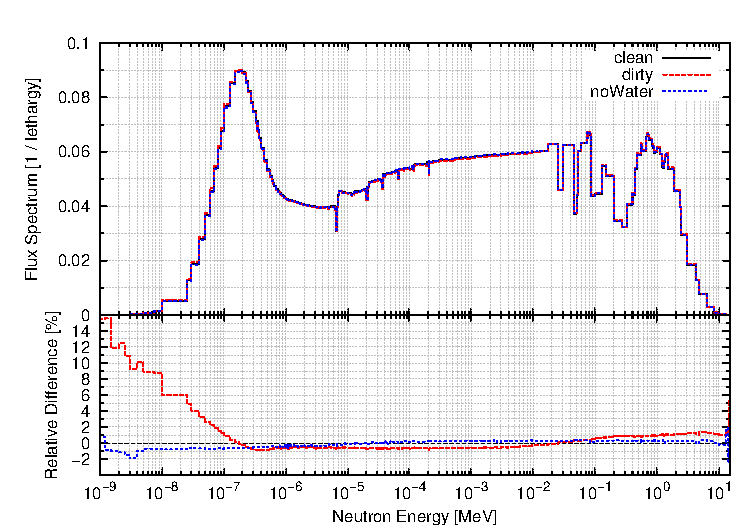
\includegraphics[width=\textwidth]{./img/fluxSpectra.pdf}
  \caption{Comparison of neutron flux spectra within clean and contaminated salts: (top) absolute value and (bottom) relative difference.}
  \label{fig:fluxSpectra}
\end{figure}

\clearpage
\begin{table}[ht]\footnotesize
    \centering
    \caption{Thermal poison equivalents of 53 flibe impurities to $0.1wppm$ \iso{Li}{6}.}
    \label{tab:thermalLimits}
    \begin{tabular}{| c | c |} \hline
    \textbf{Impurity} & \textbf{Thermal Poison} \\
                     &  \textbf{Equivalent ($w/w \E{6}$)} \\ \hline
    Zr               & $1097.59$ \\ \hline
    \water{}         & $1000.00$\footnote{MSRE concentration limit} \\ \hline
    Mg               &  $858.73$ \\ \hline
    Rb               &  $500.64$ \\ \hline
    Ce               &  $495.05$ \\ \hline
    Si               &  $365.59$ \\ \hline
    Al               &  $259.78$ \\ \hline
    Ba               &  $254.73$ \\ \hline
    Ca               &  $217.52$ \\ \hline
    U                &  $197.22$ \\ \hline
    Y                &  $154.57$ \\ \hline
    Sr               &  $152.36$ \\ \hline
    S                &  $135.39$ \\ \hline
    Zn               &  $131.14$ \\ \hline
    Na               &   $96.52$ \\ \hline
    Mo               &   $83.74$ \\ \hline
    Th               &   $70.40$ \\ \hline
    Sb               &   $52.12$ \\ \hline
    Fe               &   $48.56$ \\ \hline
    K                &   $41.43$ \\ \hline
    As               &   $38.19$ \\ \hline
    Cr               &   $37.70$ \\ \hline
    Cu               &   $37.42$ \\ \hline
    La               &   $34.35$ \\ \hline
    Ni               &   $29.10$ \\ \hline
    Pr               &   $27.29$ \\ \hline
    Br               &   $25.78$ \\ \hline
    V                &   $22.28$ \\ \hline
    W                &   $22.20$ \\ \hline
    Ta               &   $19.55$ \\ \hline
    Ti               &   $17.50$ \\ \hline
    Tb               &   $15.15$ \\ \hline
    Se               &   $15.02$ \\ \hline
    Yb               &   $11.04$ \\ \hline
    Cs               &    $9.73$ \\ \hline
    Mn               &    $9.15$ \\ \hline
    Nd               &    $6.42$ \\ \hline
    Ho               &    $5.66$ \\ \hline
    Au               &    $4.42$ \\ \hline
    Hf               &    $3.82$ \\ \hline
    Sc               &    $3.68$ \\ \hline
    Tm               &    $3.58$ \\ \hline
    Co               &    $3.53$ \\ \hline
    Cl               &    $2.38$ \\ \hline
    Er               &    $2.36$ \\ \hline
    Hg               &    $1.20$ \\ \hline
    Lu               &    $1.18$ \\ \hline
    Dy               &    $0.38$ \\ \hline
    Eu               &    $0.07$ \\ \hline
    B                &    $0.03$ \\ \hline
    Cd               &    $0.03$ \\ \hline
    Gd               &    $0.02$ \\ \hline
    Sm               &    $0.02$ \\ \hline
    \end{tabular}
\end{table}

\clearpage
\begin{table}[ht]\footnotesize
    \centering
    \caption{Specific reactivity worths of 52 flibe impurities, derived from sensitivity analysis.}
    \label{tab:sensitivityWorths}
    \begin{tabular}{| c | c |} \hline
    \textbf{Impurity} & \textbf{Specific} \\
                      & \textbf{Reactivity Worth} \\
                      & \textbf{($\Delta\rho \E{5}$) $\div$ ($w/w \E{6}$)} \\ \hline
    \water{}          &   $+0.31099\pm0.02752$ \\ \hline
    Mg                &   $+0.00261\pm0.00488$ \\ \hline
    Ce                &   $-0.00568\pm0.00326$ \\ \hline
    Zr                &   $-0.01057\pm0.00309$ \\ \hline
    Al                &   $-0.01681\pm0.00583$ \\ \hline
    S                 &   $-0.01930\pm0.00751$ \\ \hline
    Ca                &   $-0.03162\pm0.00649$ \\ \hline
    Y                 &   $-0.03452\pm0.00849$ \\ \hline
    Ba                &   $-0.03695\pm0.00413$ \\ \hline
    Rb                &   $-0.04326\pm0.00512$ \\ \hline
    Na                &   $-0.04927\pm0.02269$ \\ \hline
    Zn                &   $-0.05249\pm0.01219$ \\ \hline
    Fe                &   $-0.06553\pm0.02125$ \\ \hline
    V                 &   $-0.07110\pm0.04371$ \\ \hline
    Cr                &   $-0.07826\pm0.01907$ \\ \hline
    Sr                &   $-0.08643\pm0.00960$ \\ \hline
    K                 &   $-0.08661\pm0.01298$ \\ \hline
    Ti                &   $-0.09404\pm0.03187$ \\ \hline
    La                &   $-0.12210\pm0.01513$ \\ \hline
    Ni                &   $-0.12643\pm0.04221$ \\ \hline
    Cu                &   $-0.13019\pm0.02279$ \\ \hline
    Pr                &   $-0.16686\pm0.02122$ \\ \hline
    Mo                &   $-0.16709\pm0.01144$ \\ \hline
    Si                &   $-0.18332\pm0.03337$ \\ \hline
    Se                &   $-0.21330\pm0.03610$ \\ \hline
    Th                &   $-0.25632\pm0.00888$ \\ \hline
    Mn                &   $-0.37889\pm0.07251$ \\ \hline
    Nd                &   $-0.49841\pm0.06399$ \\ \hline
    As                &   $-0.54602\pm0.01685$ \\ \hline
    Br                &   $-0.70079\pm0.02499$ \\ \hline
    Sb                &   $-0.79432\pm0.01355$ \\ \hline
    Tm                &   $-0.90096\pm0.13574$ \\ \hline
    Sc                &   $-0.90096\pm0.13574$ \\ \hline
    W                 &   $-1.11602\pm0.04552$ \\ \hline
    Cl                &   $-1.39413\pm0.15205$ \\ \hline
    Co                &   $-1.49157\pm0.11047$ \\ \hline
    Tb                &   $-1.56372\pm0.02950$ \\ \hline
    Cs                &   $-1.96225\pm0.03172$ \\ \hline
    Yb                &   $-1.96225\pm0.03172$ \\ \hline
    Hg                &   $-2.07514\pm0.10698$ \\ \hline
    Ta                &   $-2.32961\pm0.02111$ \\ \hline
    Ho                &   $-2.63395\pm0.05047$ \\ \hline
    Lu                &   $-3.41424\pm0.11040$ \\ \hline
    Au                &   $-4.84578\pm0.04973$ \\ \hline
    Hf                &   $-6.70753\pm0.09079$ \\ \hline
    Er                &   $-7.13363\pm0.06575$ \\ \hline
    Dy                &  $-10.93813\pm0.31960$ \\ \hline
    Eu                &  $-49.62564\pm0.52968$ \\ \hline
    Cd                &  $-78.10976\pm0.50762$ \\ \hline
    Sm                &  $-96.82404\pm1.70144$ \\ \hline
    B                 & $-101.05397\pm1.31990$ \\ \hline
    Gd                & $-164.47373\pm0.30358$ \\ \hline
    \end{tabular}
\end{table}

\clearpage
\begin{table}[ht]\footnotesize
    \centering
    \caption{Specific reactivity worths of $50wppm$ \iso{Li}{6} flibe components, derived from sensitivity analysis.}
    \label{tab:flibeWorths}
    \begin{tabular}{| c | c |} \hline
    \textbf{Impurity} & \textbf{Specific} \\
                      & \textbf{Reactivity Worth} \\
                      & \textbf{($\Delta\rho \E{5}$) $\div$ ($w/w \E{6}$)} \\ \hline
    Be                & $+0.02215\pm0.00085$ \\ \hline
    Be + F            & $+0.00315\pm0.00023$ \\ \hline
    F                 & $+0.00090\pm0.00024$ \\ \hline
    flibe             & $+0.00061\pm0.00021$ \\ \hline
    Li + Be           & $-0.00035\pm0.00042$ \\ \hline
    Li + F            & $-0.00155\pm0.00021$ \\ \hline
    Li                & $-0.01480\pm0.00042$ \\ \hline
    \end{tabular}
\end{table}

\clearpage
\begin{table}[ht]\footnotesize
    \centering
    \caption{Specific reactivity worths of 53 impurities and flibe, derived from spectrum-collapsed absorption cross-sections.}
    \label{tab:absorptionWorths}
    \begin{tabular}{| c | c |} \hline
    \textbf{Impurity} & \textbf{Specific} \\
                      & \textbf{Reactivity Worth} \\
                      & \textbf{($\Delta\rho \E{5}$) $\div$ ($w/w \E{6}$)} \\ \hline
    Mg                &   $-0.00315\pm0.00000$ \\ \hline
    Ce                &   $-0.00590\pm0.00000$ \\ \hline
    Si                &   $-0.00709\pm0.00000$ \\ \hline
    Zr                &   $-0.00857\pm0.00000$ \\ \hline
    Al                &   $-0.01005\pm0.00000$ \\ \hline
    Ca                &   $-0.01431\pm0.00000$ \\ \hline
    Y                 &   $-0.01752\pm0.00000$ \\ \hline
    S                 &   $-0.02285\pm0.00000$ \\ \hline
    Na                &   $-0.02707\pm0.00001$ \\ \hline
    Zn                &   $-0.03739\pm0.00001$ \\ \hline
    \water{}          &   $-0.04029\pm0.00001$ \\ \hline
    Ba                &   $-0.04114\pm0.00001$ \\ \hline
    Rb                &   $-0.04783\pm0.00001$ \\ \hline
    Fe                &   $-0.05188\pm0.00001$ \\ \hline
    Sr                &   $-0.05778\pm0.00001$ \\ \hline
    K                 &   $-0.06275\pm0.00002$ \\ \hline
    Cr                &   $-0.06515\pm0.00001$ \\ \hline
    Ni                &   $-0.08404\pm0.00002$ \\ \hline
    Cu                &   $-0.08762\pm0.00002$ \\ \hline
    La                &   $-0.10172\pm0.00003$ \\ \hline
    V                 &   $-0.11213\pm0.00003$ \\ \hline
    Ti                &   $-0.13965\pm0.00003$ \\ \hline
    Pr                &   $-0.14181\pm0.00002$ \\ \hline
    Mo                &   $-0.16468\pm0.00005$ \\ \hline
    Th                &   $-0.22220\pm0.00006$ \\ \hline
    Se                &   $-0.22704\pm0.00004$ \\ \hline
    Mn                &   $-0.32696\pm0.00005$ \\ \hline
    Nd                &   $-0.44026\pm0.00008$ \\ \hline
    U                 &   $-0.45322\pm0.00016$ \\ \hline
    As                &   $-0.52930\pm0.00014$ \\ \hline
    Tm                &   $-0.65501\pm0.00017$ \\ \hline
    Sc                &   $-0.65501\pm0.00017$ \\ \hline
    Br                &   $-0.69553\pm0.00015$ \\ \hline
    Sb                &   $-0.69915\pm0.00016$ \\ \hline
    W                 &   $-0.99836\pm0.00022$ \\ \hline
    Cl                &   $-1.02814\pm0.00027$ \\ \hline
    Co                &   $-1.25807\pm0.00020$ \\ \hline
    Tb                &   $-1.41209\pm0.00037$ \\ \hline
    Cs                &   $-1.59669\pm0.00042$ \\ \hline
    Yb                &   $-1.59669\pm0.00042$ \\ \hline
    Hg                &   $-1.70078\pm0.00043$ \\ \hline
    flibe             &   $-1.83377\pm0.00048$ \\ \hline
    Ta                &   $-1.96556\pm0.00052$ \\ \hline
    Ho                &   $-2.28664\pm0.00060$ \\ \hline
    Lu                &   $-2.89198\pm0.00041$ \\ \hline
    Au                &   $-3.80139\pm0.00138$ \\ \hline
    Er                &   $-5.44962\pm0.00085$ \\ \hline
    Hf                &   $-5.56649\pm0.00112$ \\ \hline
    Dy                &   $-8.41116\pm0.00122$ \\ \hline
    Eu                &  $-38.31542\pm0.00927$ \\ \hline
    Cd                &  $-58.78493\pm0.01542$ \\ \hline
    Sm                &  $-72.48603\pm0.01818$ \\ \hline
    B                 &  $-82.90026\pm0.02179$ \\ \hline
    Gd                & $-120.55738\pm0.02644$ \\ \hline
    \end{tabular}
\end{table}

\clearpage
\begin{table}[ht]\footnotesize
    \centering
    \caption{Required impurity detection and removal precisions of 53 impurities, for a $-20pcm$ maximum reactivity penalty.}
    \label{tab:precision}
    \begin{tabular}{| c | c |} \hline
    \textbf{Precision}     & \\
    \textbf{($w/w \E{6}$)} & \textbf{Impurities} \\ \hline
    $0.1$                  & B, Cd, Sm, Eu, Gd \\ \hline
    $1$                    & Dy, Ho, Er, Lu, Hf, Ta, Au, Hg \\ \hline
    $10$                   & Cl, Sc, Mn, Co, As, Se, Br, Mo, Sb, Cs, Nd, Tb, Tm, Yb, W, Th, U \\ \hline
    $100$                  & \water{}, Na, S, K, Ti, V, Cr, Fe, Ni, Cu, Zn, Rb, Sr, Y, Ba, La, Pr \\ \hline
    $1000$                 & Mg, Al, Si, Ca, Zr, Ce \\ \hline
    \end{tabular}
\end{table}

\clearpage
\begin{table}[ht]\footnotesize
    \centering
    \caption{Concentration and reactivity worth of 43 flibe impurities, measured by delayed gamma neutron activation analysis.}
    \label{tab:concentration}
    \begin{tabular}{| c | c | c |} \hline
    \textbf{Impurity} & \textbf{Concentration} & \textbf{Estimated Reactivity} \\
                      & \textbf{($w/w \E{6}$)} & \textbf{Worth ($\Delta\rho \E{5}$)} \\ \hline
    Mg                & $110.$                 &   $+0.28679\pm0.53697$ \\ \hline
    Au                & $< 0.00037$            &   $-0.00179\pm0.00002$ \\ \hline
    Ce                &   $0.389$              &   $-0.00221\pm0.00127$ \\ \hline
    La                &   $0.07$               &   $-0.00855\pm0.00106$ \\ \hline
    Lu                & $< 0.0037$             &   $-0.01263\pm0.00041$ \\ \hline
    Th                &   $0.072$              &   $-0.01846\pm0.00064$ \\ \hline
    Br                &   $0.033$              &   $-0.02313\pm0.00082$ \\ \hline
    Sb                &   $0.038$              &   $-0.03018\pm0.00051$ \\ \hline
    Sc                &   $0.035$              &   $-0.03153\pm0.00475$ \\ \hline
    U                 & $< 0.083$              &   $-0.03762\pm0.00001$ \\ \hline
    Tb                & $< 0.031$              &   $-0.04848\pm0.00091$ \\ \hline
    V                 &   $0.72$               &   $-0.05119\pm0.03147$ \\ \hline
    Yb                & $< 0.034$              &   $-0.06672\pm0.00108$ \\ \hline
    Rb                &   $1.7$                &   $-0.07354\pm0.00870$ \\ \hline
    Se                & $< 0.4$                &   $-0.08532\pm0.01444$ \\ \hline
    Zn                &   $1.89$               &   $-0.09920\pm0.02303$ \\ \hline
    Zr                &   $9.5$                &   $-0.10044\pm0.02931$ \\ \hline
    Mo                &   $0.66$               &   $-0.11028\pm0.00755$ \\ \hline
    W                 &   $0.152$              &   $-0.16963\pm0.00692$ \\ \hline
    Cr                &   $2.42$               &   $-0.18939\pm0.04616$ \\ \hline
    Ba                &   $5.5$                &   $-0.20320\pm0.02269$ \\ \hline
    Sm                & $< 0.0026$             &   $-0.25174\pm0.00442$ \\ \hline
    Hf                & $< 0.043$              &   $-0.28842\pm0.00390$ \\ \hline
    Dy                & $< 0.03$               &   $-0.32814\pm0.00959$ \\ \hline
    Hg                & $< 0.16$               &   $-0.33202\pm0.01712$ \\ \hline
    Co                &   $0.24$               &   $-0.35798\pm0.02651$ \\ \hline
    Al                & $ 30.$                 &   $-0.50420\pm0.17489$ \\ \hline
    Sr                &   $ 7.34$              &   $-0.63438\pm0.07045$ \\ \hline
    Mn                &   $ 1.81$              &   $-0.68579\pm0.13123$ \\ \hline
    Fe                &   $12.7$               &   $-0.83223\pm0.26986$ \\ \hline
    Nd                & $<  2.1$               &   $-1.04666\pm0.13437$ \\ \hline
    Ta                & $<  0.49$              &   $-1.14151\pm0.01035$ \\ \hline
    As                &   $ 2.27$              &   $-1.23946\pm0.03825$ \\ \hline
    Eu                &   $ 0.03$              &   $-1.48877\pm0.01589$ \\ \hline
    Cs                &   $ 1.16$              &   $-2.27621\pm0.03679$ \\ \hline
    Cu                & $< 22.$                &   $-2.86416\pm0.50132$ \\ \hline
    Ca                & $<115.$                &   $-3.63684\pm0.74670$ \\ \hline
    Ti                & $< 57.$                &   $-5.36012\pm1.81672$ \\ \hline
    Ni                &   $63.6$               &   $-8.04113\pm2.68471$ \\ \hline
    Na                & $ 209.$                &  $-10.29686\pm4.74132$ \\ \hline
    K                 & $ 272.$                &  $-23.55851\pm3.53106$ \\ \hline
    Cl                &   $35.$                &  $-48.79451\pm5.32166$ \\ \hline
    Cd                & $<  0.73$              &  $-57.02013\pm0.37056$ \\ \hline
    Total             & $-$                    & $-172.05646\pm8.66975$ \\ \hline
    \end{tabular}
\end{table}

\clearpage
\begin{table}[ht]\footnotesize
    \centering
    \caption{Spectrochemical analysis of MSRE flush salt during initial use.}
    \label{tab:detection}
    \begin{tabular}{| c |}
    \end{tabular}
\end{table}

\end{document}
